% fancytikzposter.tex, version 2.1
% Original template created by Elena Botoeva [botoeva@inf.unibz.it], June 2012
% 
% This file is distributed under the Creative Commons Attribution-NonCommercial 2.0
% Generic (CC BY-NC 2.0) license
% http://creativecommons.org/licenses/by-nc/2.0/ 


\documentclass{a0poster}

\usepackage{fancytikzposter} 

\usepackage{tikz}
\usetikzlibrary{arrows,positioning,automata,shadows,fit,shapes}
\tikzstyle{block} = [rectangle, draw, fill=blue!20, 
    text width=6em, text centered, rounded corners, minimum height=4em]
    \tikzstyle{line} = [draw, -latex']
\usepackage{graphicx}
\usepackage[english]{babel}
\usepackage{multirow}
\usepackage{algpseudocode}
\usepackage[labelformat=empty]{caption}
\usepackage{ulem}
\usepackage{caption}
\usepackage{xcolor,colortbl}
\usepackage{multicol}
\usepackage{graphics}
\usepackage{color}

\usepackage[12pt]{moresize}

\definecolor{yellow}{HTML}{FFCC00}
\definecolor{pink}{HTML}{FF33CC}

\algtext*{EndIf}% Remove "end if" text
\algtext*{EndFor}% Remove "end if" text

\graphicspath{{images/}}

\usepackage{amsthm}
\newtheorem*{definition*}{Definition}
\newtheorem{definition}{Definition}

%%%%% --------- Change here if you want ---------- %%%%%
%% margin for the geometry package, must be changed before using the geometry package
%% default value is 4cm
% \setmargin{4}

%% the space between the blocks
%% default value is 2cm
% \setblockspacing{2}

%% the height of the title stripe in block nodes, decrease it to save space
%% default value is 3cm
% \setblocktitleheight{3}

%% the number of columns in the poster, possible values 2,3
%% default value is 2
% \setcolumnnumber{3}

%% the space between two or more groups of authors from different institutions
%% used in \maketitle
% \setinstituteshift{10}

%% which template to use
%% N1 simple, standard look, with a colored background and gray boxes
%% N2 board with nodes
%% N3 another standard look
%% N4 envelope-like look
%% N5 with a wave-like head, original idea taken from
%%%% http://fc09.deviantart.net/fs71/f/2010/322/1/1/scientific_poster_by_nabuy-d333ria.jpg
%\usetemplate{6}

%% components of the templates
%% (the maximal possible numbers are mentioned as the parameters)
% \usecolortemplate{4}
% \usebackgroundtemplate{5}
% \usetitletemplate{2}
% \useblocknodetemplate{5}
% \useplainblocktemplate{4}
% \useinnerblocktemplate{2}


%% the height of the head drawing on top 
%% applicable to templates N3, 4 and 5
% \setheaddrawingheight{14}


%% change the basic colors
%\definecolor{myblue}{HTML}{008888} 
%\setfirstcolor{myblue}% default 116699
%\setsecondcolor{gray!80!}% default CCCCCC
%\setthirdcolor{red!80!black}% default 991111

%% change the more specific colors
% \setbackgrounddarkcolor{colorone!70!black}
% \setbackgroundlightcolor{colorone!70!}
% \settitletextcolor{textcolor}
% \settitlefillcolor{white}
% \settitledrawcolor{colortwo}
% \setblocktextcolor{textcolor}
% \setblockfillcolor{white}
% \setblocktitletextcolor{colorone}
% \setblocktitlefillcolor{colortwo} %the color of the border
% \setplainblocktextcolor{textcolor}
% \setplainblockfillcolor{colorthree!40!}
% \setplainblocktitletextcolor{textcolor}
% \setplainblocktitlefillcolor{colorthree!60!}
% \setinnerblocktextcolor{textcolor}
% \setinnerblockfillcolor{white}
% \setinnerblocktitletextcolor{white}
% \setinnerblocktitlefillcolor{colorthree}




%%% size of the document and the margins
%% A0
% \usepackage[margin=\margin cm, paperwidth=118.9cm, paperheight=84.1cm]{geometry} 
\usepackage[margin=\margin cm, paperwidth=84.1cm, paperheight=118.9cm]{geometry}
%% B1
% \usepackage[margin=\margin cm, paperwidth=70cm, paperheight=100cm]{geometry}



%% changing the fonts
\usepackage{cmbright}
%\usepackage[default]{cantarell}
%\usepackage{avant}
%\usepackage[math]{iwona}
\usepackage[math]{kurier}
\usepackage[T1]{fontenc}


%% add your packages here
\usepackage{hyperref}





\title{Using Reachability Properties of Logic Program for Revising Biological Models}
\author{Xinwei Chai$^{1,2}$, Tony Ribeiro$^{1,2}$, Morgan Magnin$^{1,2}$, Olivier Roux$^{1}$ and Katsumi Inoue$^{2}$\\
	$^1$Laboratoire des Sciences du Num\'erique de Nantes, France\\
	$^2$National Institute of Informatics, Japan\\
	{\small \texttt{\{xinwei.chai, tony.ribeiro, morgan.magnin, olivier.roux\}@ls2n.fr}, \texttt{inoue@nii.ac.jp}}
}



\begin{document}

%%%%% ---------- the background picture ---------- %%%%%
%% to change it modify the macro \BackgroundPicture
\ClearShipoutPicture
\AddToShipoutPicture{\BackgroundPicture}

\noindent % to have the picture right in the center
\begin{tikzpicture}
  \initializesizeandshifts
  % \setxshift{15}
  % \setyshift{2}


  %% the title block, #1 - shift, the default value is (0,0), #2 - width, #3 - scale
  %% the alias of the title block is `title', so we can refer to its boundaries later
  \ifthenelse{\equal{\template}{1}}{ 
    \titleblock{47}{1}
  }{
    \titleblock{47}{1.5}
  }

  %% a logo can be added to the title block
  %% #1 - anchor relative to the title block, #2 - shift, #3 - width, #3 - file name
  % \ifthenelse{\equal{\template}{2}}{ 
  %   \addlogo[south west]{(2,0)}{6cm}{unibz_b.png}
  % }{
  %   \addlogo[south west]{(2,0)}{6cm}{unibz_w.png}
  % }


  %% a block node, with the specified position (optional), title and the content
  %% #1 - where (optional), #2 - title, #3 - text
  %%%%%%%%%% ------------------------------------------ %%%%%%%%%%
  \blocknode%
  {Motivation}%
  {
  \begin{itemize}
      \item We can learn a model from biological data but do not know if it is consistent with background knowledge
  \end{itemize}
  	\innerblockplain[colorone!80!]{
  		\center
  			\begin{picture}(35,10)
			    \put(0,-3.5){\hbox{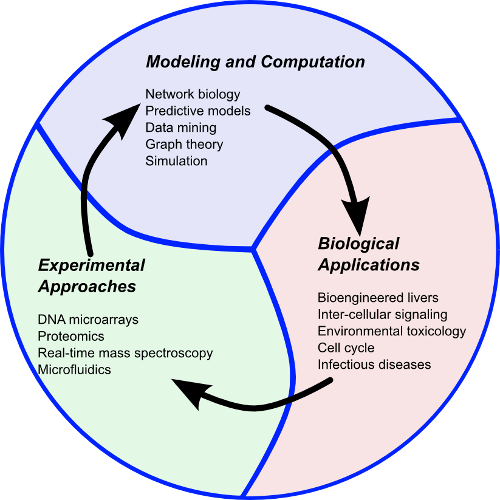
\includegraphics[keepaspectratio=true,width=0.4\textwidth]{systems_biology.png}}}
			    \put(15,-2){\hbox{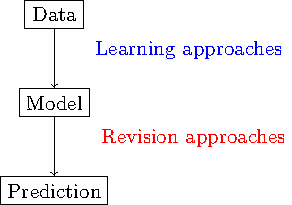
\includegraphics[keepaspectratio=true,width=0.4\textwidth]{bigPicture.pdf}
			    }}
			\end{picture}
			
			\vspace{3.5cm}
	}
	
	
  }
  
  \blocknode%
  {Methodology}%
  {
  	\centering
  
  	\begin{picture}(31,20)
		\put(0,1.75){\hbox{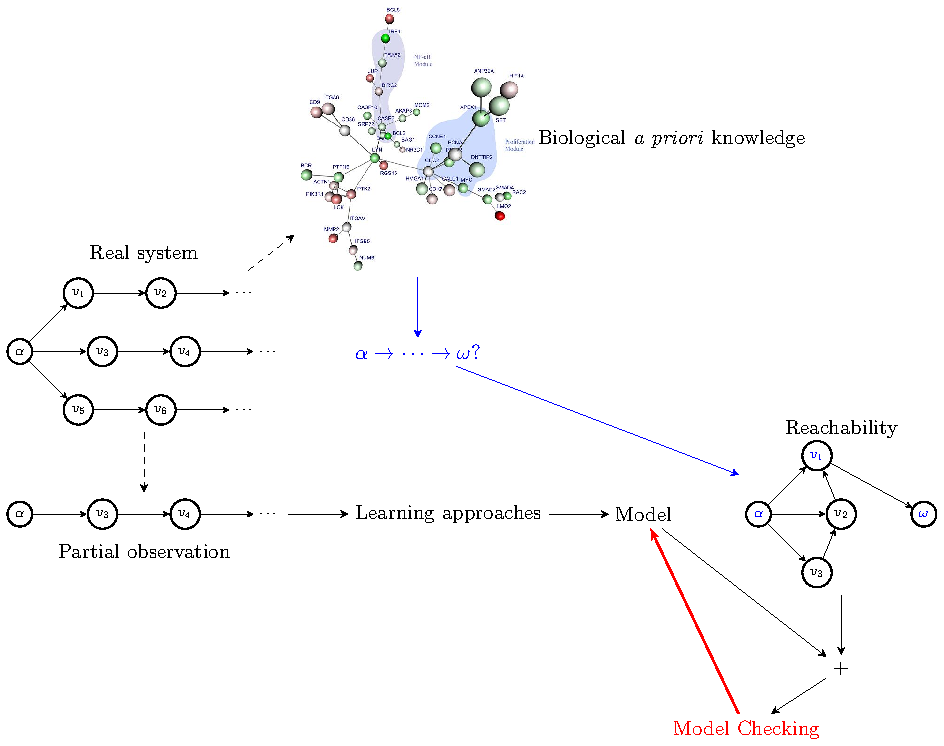
\includegraphics[scale=1.5]{scheme.pdf}}}
	\end{picture}
		
  }
  
  
  \blocknode%
  {LCG: Local Causality Graph}%
  {
  Start with target state $\omega\to$ Find transitions reaching $\omega\to$ Find new target states to fire those transitions $\to\cdots$ Recursion $\cdots\to$ End with initial state $\alpha$

\begin{itemize}
\item Goal-oriented structure 
\item Formed by recursive updates
%starting with desired final state, for each update, link the states with their associated transitions if they are not at initial state. Update ends when the graph becomes saturated.
\item Avoid global search in state transition graphs
\end{itemize}
	\begin{picture}(30,12)
		\put(3,10){\hbox{Rules: $a_1\gets \{b_1, c_1\}$, 
        $a_1\gets e_1$,

        $b_1\gets d_0$, 
        $c_1\gets d_1$, 
        $d_1\gets b_1$}}
		\put(3,2){\hbox{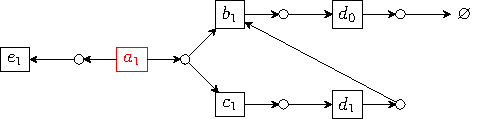
\includegraphics[width=0.8\textwidth]{lcg.pdf}}}
		\put(3,0){\hbox{Learned Network and correpsonding LCG for studying the reachability of $a_1$}}
	\end{picture}
  }
  
  \startsecondcolumn
  
  \blocknode%
  {Learning From Interpretation Transition (LFIT)}%
  {
  	\centering
  	
	
	\begin{picture}(30,6)
		
	\end{picture}
  }

  

  \blocknode%
  {Model Revision based on Model Checking}%
  {
\begin{itemize}
    \item By adding elements in the body of a transition, it is possible to change a reachable state to an unreachable one
    \item By deleting elements in the body of a transition, it is possible to change an unreachable state to a reachable one
\end{itemize}

	\centering
	
	\begin{picture}(30,10)
        \put(3,1){\hbox{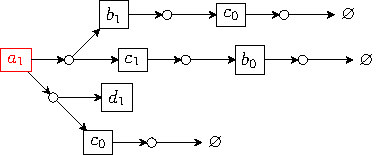
\includegraphics[width=0.6\textwidth]{completionSet.pdf}}}
        \put(3,0){\hbox{Example of generalization}}


	\end{picture}
	
    \begin{itemize}
        \item $L=\{\{(\alpha,a_1)\}\}$
        \item $a_1$ is reachable if (1)$\{b_1,c_1\}\to a_0\Rsh a_1$ or (2)$\{c_0,d_1\}\to a_0\Rsh a_1$ is generalized
        \item (1) can only be generalized to $\{b_1\}\to a_0\Rsh a_1$ as $c_1\in U_K$
        \item (2) can only be generalized to $\{c_0\}\to a_0\Rsh a_1$ as $d_1\in U_K$
        \item Check the reachability of $a_1$, reachable, finish
    \end{itemize}
  }
  
  \blocknode%
  {Evaluation of Reachability Analyzers}%
  { \small
  \centering
  \begin{tabular}{|c|c|c|c|c|c|c|c|c|c|}
    \hline
  	Model	&\multicolumn{3}{c|}{$\lambda$-phage}	&	  \multicolumn{3}{c|}{TCR} & \multicolumn{3}{c|}{EGFR}  \\
    \hline
    Inputs&\multicolumn{3}{c|}{4}	&	  \multicolumn{3}{c|}{3} & \multicolumn{3}{c|}{13}\\
    \hline
    Outputs&\multicolumn{3}{c|}{4} &	  \multicolumn{3}{c|}{5} & \multicolumn{3}{c|}{12} \\
    \hline
    Total tests&\multicolumn{3}{c|}{$2^4\times 4=64$} & \multicolumn{3}{c|}{$2^3\times 5=40$} & \multicolumn{3}{c|}{$2^{13}\times 12=98,304$}\\
    \hline
    Analyzer  &  Pint  &  \textbf{PR}   &\textbf{AR}    &  Pint  &  \textbf{PR}     &\textbf{AR}   &  Pint  &  \textbf{PR}     &\textbf{AR}             \\
    \hline
    Reachable    & 36(56\%)& 38(59\%)& 38(59\%)   &  \multicolumn{3}{c|}{16(40\%)}  & 64,282(65.4\%)  & \multicolumn{2}{c|}{74,268(75.5\%)}\\
    \hline
    \textbf{Inconclusive} & \textcolor{red}{\textbf{2(3\%)}}&\multicolumn{2}{c|}{\textcolor{blue}{\textbf{0(0\%)}}}& \multicolumn{3}{c|}{0(0\%)}    &\textcolor{red}{\textbf{9,986(10.1\%)}}&\multicolumn{2}{c|}{\textcolor{blue}{\textbf{0(0\%)}}}  \\
    \hline
    Unreachable     &  \multicolumn{3}{c|}{26(41\%)} &  \multicolumn{3}{c|}{24(60\%)} &\multicolumn{3}{c|}{24,036(24.5\%)}\\
    \hline
    Total time &  \multicolumn{3}{c|}{$<1$s}        &  7s     &0.85s  &  40s        & \textbf{9h50min}      & \textbf{15min31s}         & \textbf{3h46min}      \\
    \hline
    \end{tabular}
    
    PR=PermReach, AR=ASPReach
    
    Tests are carried on a computer of Intel Core i7-3770 CPU, \@3.4GHz, 8.00G RAM. 
Results of the tests on small ($\lambda$-phage) and large (TCR,EGFR) examples from biology literature. 
Results of model-checkers using global search are memory-out so are not listed in the table.
``Reachable", ``Inconclusive" and ``Unreachable" give respectively the number of different results of reachability, while “Max time” and “Total time” depict respectively the maximum time of the individual computations..
Column “Pint” gives the related results on ANs, while column “PermReach” gives the results for ABANs. 
    
    
	
%	\begin{picture}(35,14)
%			\put(3,0){\hbox{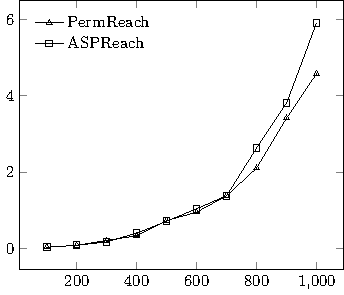
\includegraphics[width=0.4\textwidth]{sizeTest.pdf}}}
%		\put(18,0){\hbox{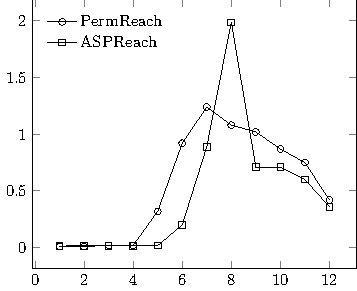
\includegraphics[width=0.4\textwidth]{inconcTest.pdf}}}
%	\end{picture}
	
		Performance test on randomly generated examples
	
  }


\end{tikzpicture}


\end{document}




